%\pdfoutput=0
\documentclass[twocolumn]{article}
\usepackage{graphicx}
\title{An example of using \LaTeX{} and Gnuplot: the exponential function}
\author{D.V.~Fedorov}
\begin{document}
\maketitle

\noindent
The exponential function can be defined as the solution to the
differential equaion,
\begin{equation}\label{diff-eq}
y'(x)=y(x) \;,
\end{equation}
with the boundary condition
\begin{equation}\label{bound-cond}
y(0)=1 \;.
\end{equation}

The argument can be reduced to $x\in[0,1]$ using identities,
\begin{eqnarray}
\exp(x)&=&\exp\left(\frac{x}{2}\right)\exp\left(\frac{x}{2}\right) \;, \\
\exp(-x)&=&\frac{1}{\exp(x)} \;.
\end{eqnarray}

Once the argument is reduced, the differential equation~(\ref{diff-eq})
can be integrated numerically with sufficient accuracy.

\begin{figure}[h]
% GNUPLOT: LaTeX picture with Postscript
\begingroup
  \makeatletter
  \providecommand\color[2][]{%
    \GenericError{(gnuplot) \space\space\space\@spaces}{%
      Package color not loaded in conjunction with
      terminal option `colourtext'%
    }{See the gnuplot documentation for explanation.%
    }{Either use 'blacktext' in gnuplot or load the package
      color.sty in LaTeX.}%
    \renewcommand\color[2][]{}%
  }%
  \providecommand\includegraphics[2][]{%
    \GenericError{(gnuplot) \space\space\space\@spaces}{%
      Package graphicx or graphics not loaded%
    }{See the gnuplot documentation for explanation.%
    }{The gnuplot epslatex terminal needs graphicx.sty or graphics.sty.}%
    \renewcommand\includegraphics[2][]{}%
  }%
  \providecommand\rotatebox[2]{#2}%
  \@ifundefined{ifGPcolor}{%
    \newif\ifGPcolor
    \GPcolortrue
  }{}%
  \@ifundefined{ifGPblacktext}{%
    \newif\ifGPblacktext
    \GPblacktexttrue
  }{}%
  % define a \g@addto@macro without @ in the name:
  \let\gplgaddtomacro\g@addto@macro
  % define empty templates for all commands taking text:
  \gdef\gplbacktext{}%
  \gdef\gplfronttext{}%
  \makeatother
  \ifGPblacktext
    % no textcolor at all
    \def\colorrgb#1{}%
    \def\colorgray#1{}%
  \else
    % gray or color?
    \ifGPcolor
      \def\colorrgb#1{\color[rgb]{#1}}%
      \def\colorgray#1{\color[gray]{#1}}%
      \expandafter\def\csname LTw\endcsname{\color{white}}%
      \expandafter\def\csname LTb\endcsname{\color{black}}%
      \expandafter\def\csname LTa\endcsname{\color{black}}%
      \expandafter\def\csname LT0\endcsname{\color[rgb]{1,0,0}}%
      \expandafter\def\csname LT1\endcsname{\color[rgb]{0,1,0}}%
      \expandafter\def\csname LT2\endcsname{\color[rgb]{0,0,1}}%
      \expandafter\def\csname LT3\endcsname{\color[rgb]{1,0,1}}%
      \expandafter\def\csname LT4\endcsname{\color[rgb]{0,1,1}}%
      \expandafter\def\csname LT5\endcsname{\color[rgb]{1,1,0}}%
      \expandafter\def\csname LT6\endcsname{\color[rgb]{0,0,0}}%
      \expandafter\def\csname LT7\endcsname{\color[rgb]{1,0.3,0}}%
      \expandafter\def\csname LT8\endcsname{\color[rgb]{0.5,0.5,0.5}}%
    \else
      % gray
      \def\colorrgb#1{\color{black}}%
      \def\colorgray#1{\color[gray]{#1}}%
      \expandafter\def\csname LTw\endcsname{\color{white}}%
      \expandafter\def\csname LTb\endcsname{\color{black}}%
      \expandafter\def\csname LTa\endcsname{\color{black}}%
      \expandafter\def\csname LT0\endcsname{\color{black}}%
      \expandafter\def\csname LT1\endcsname{\color{black}}%
      \expandafter\def\csname LT2\endcsname{\color{black}}%
      \expandafter\def\csname LT3\endcsname{\color{black}}%
      \expandafter\def\csname LT4\endcsname{\color{black}}%
      \expandafter\def\csname LT5\endcsname{\color{black}}%
      \expandafter\def\csname LT6\endcsname{\color{black}}%
      \expandafter\def\csname LT7\endcsname{\color{black}}%
      \expandafter\def\csname LT8\endcsname{\color{black}}%
    \fi
  \fi
    \setlength{\unitlength}{0.0500bp}%
    \ifx\gptboxheight\undefined%
      \newlength{\gptboxheight}%
      \newlength{\gptboxwidth}%
      \newsavebox{\gptboxtext}%
    \fi%
    \setlength{\fboxrule}{0.5pt}%
    \setlength{\fboxsep}{1pt}%
\begin{picture}(3940.00,2800.00)%
    \gplgaddtomacro\gplbacktext{%
      \csname LTb\endcsname%%
      \put(202,630){\makebox(0,0)[r]{\strut{}$0.1$}}%
      \csname LTb\endcsname%%
      \put(202,1129){\makebox(0,0)[r]{\strut{}$1$}}%
      \csname LTb\endcsname%%
      \put(202,1627){\makebox(0,0)[r]{\strut{}$10$}}%
      \csname LTb\endcsname%%
      \put(202,2126){\makebox(0,0)[r]{\strut{}$100$}}%
      \csname LTb\endcsname%%
      \put(202,2624){\makebox(0,0)[r]{\strut{}$1000$}}%
      \csname LTb\endcsname%%
      \put(277,385){\makebox(0,0){\strut{}$-2$}}%
      \csname LTb\endcsname%%
      \put(788,385){\makebox(0,0){\strut{}$-1$}}%
      \csname LTb\endcsname%%
      \put(1299,385){\makebox(0,0){\strut{}$0$}}%
      \csname LTb\endcsname%%
      \put(1810,385){\makebox(0,0){\strut{}$1$}}%
      \csname LTb\endcsname%%
      \put(2321,385){\makebox(0,0){\strut{}$2$}}%
      \csname LTb\endcsname%%
      \put(2832,385){\makebox(0,0){\strut{}$3$}}%
      \csname LTb\endcsname%%
      \put(3343,385){\makebox(0,0){\strut{}$4$}}%
      \csname LTb\endcsname%%
      \put(3854,385){\makebox(0,0){\strut{}$5$}}%
    }%
    \gplgaddtomacro\gplfronttext{%
      \csname LTb\endcsname%%
      \put(91,1627){\rotatebox{-270}{\makebox(0,0){\strut{}$y$}}}%
      \csname LTb\endcsname%%
      \put(2065,123){\makebox(0,0){\strut{}$x$}}%
      \csname LTb\endcsname%%
      \put(362,2466){\makebox(0,0)[r]{\strut{}$\exp(x)$}}%
      \csname LTb\endcsname%%
      \put(362,2291){\makebox(0,0)[r]{\strut{}tabulated values}}%
    }%
    \gplbacktext
    \put(0,0){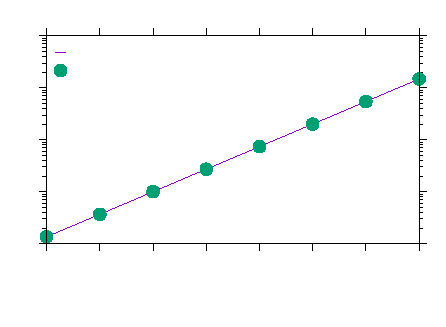
\includegraphics{plot-exp}}%
    \gplfronttext
  \end{picture}%
\endgroup

\caption{Illustration of the exponential function.}
\end{figure}

\end{document}
